\documentclass[11pt]{article}

\usepackage[margin=1.0in]{geometry}
\usepackage{tablefootnote}
\usepackage[export]{adjustbox}
\usepackage{graphicx}
\usepackage{natbib}
\usepackage{amsmath}
\usepackage{color}
\usepackage{lscape}

\pdfminorversion 4

\bibpunct[,]{(}{)}{;}{a}{}{,}
\renewcommand{\bottomfraction}{.9}
\renewcommand{\topfraction}{.9}
\renewcommand{\textfraction}{0.1}
\renewcommand{\floatpagefraction}{.9}

\begin{document}

\title{\textbf{Supplementary Information for:\\ Extensively parameterized mutation--selection models reliably capture site-specific selective constraint}}
\author{Stephanie J. Spielman$^{1,2*}$ and Claus O. Wilke$^{1}$}
\date{}

\maketitle

\noindent
Address:\\
$^1$Department of Integrative Biology, Center for Computational Biology and Bioinformatics, and Institute for Cellular and Molecular Biology. The University of Texas at Austin, Austin, TX.\\\\
Current Address:\\
$^2$Institute for Genomics and Evolutionary Medicine. Temple University, Philadelphia, PA.

\bigskip
\noindent
$^*$Corresponding author\\
$\phantom{^*}$Email: stephanie.spielman@gmail.com\\


\section*{Supplementary Figures}


\vspace*{2cm}
\centerline{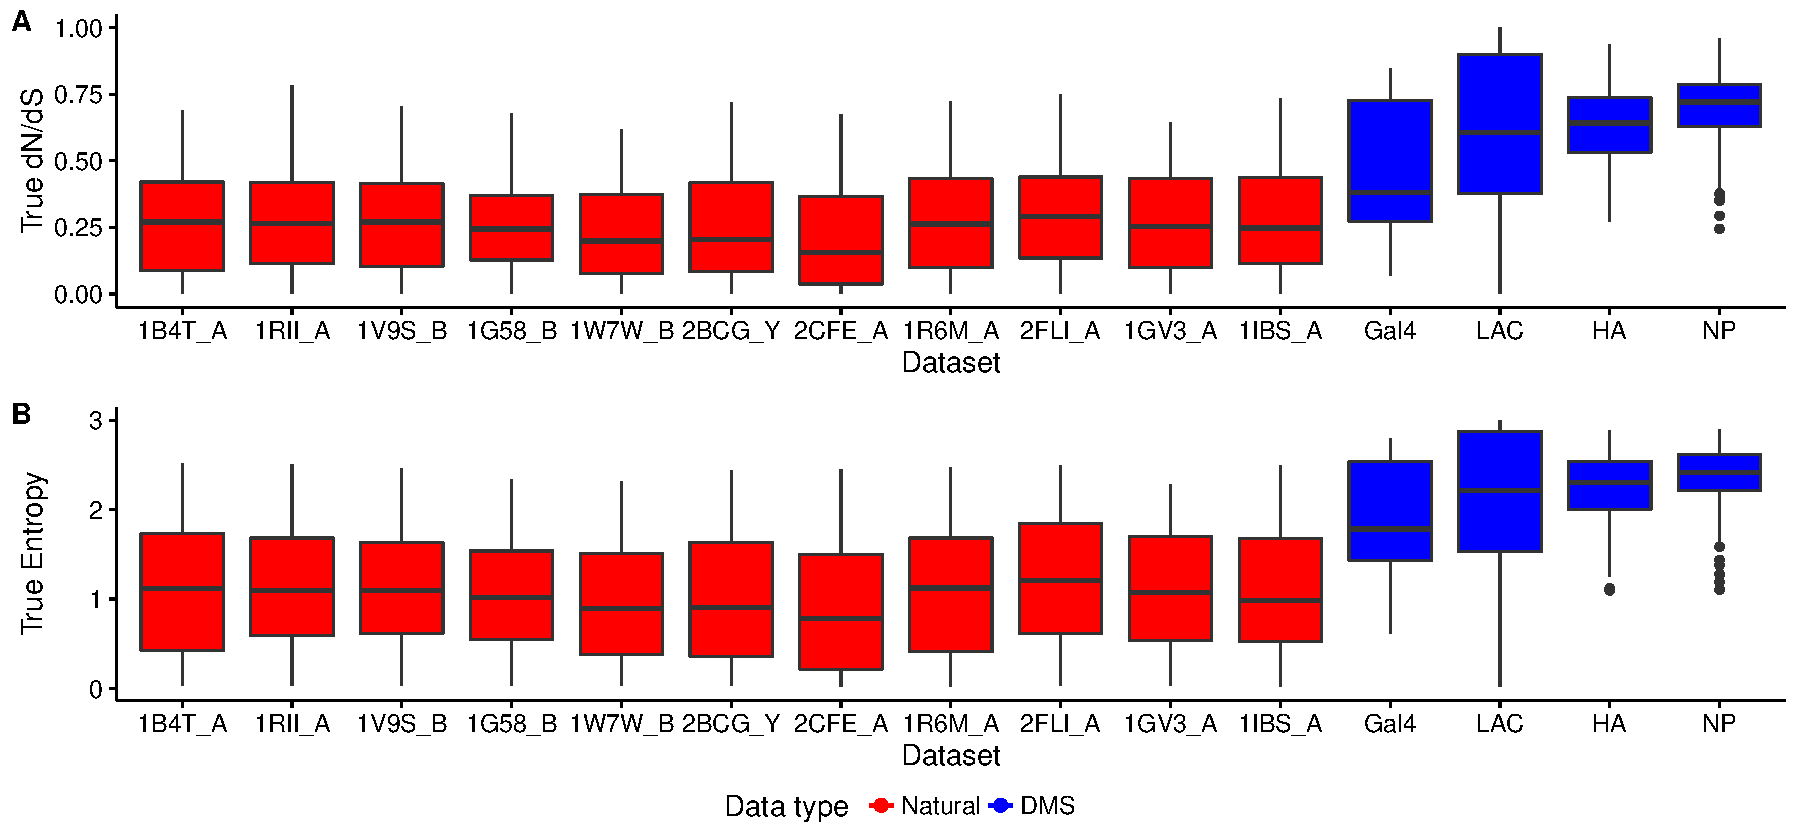
\includegraphics[width=7in]{SI_Figures/full_boxplot_dnds_entropy.pdf}}
\noindent{\textbf{Figure S1} Distributions of true site-specific $dN/dS$ and entropies across simulation parameterizations.

\vspace*{2cm}
\centerline{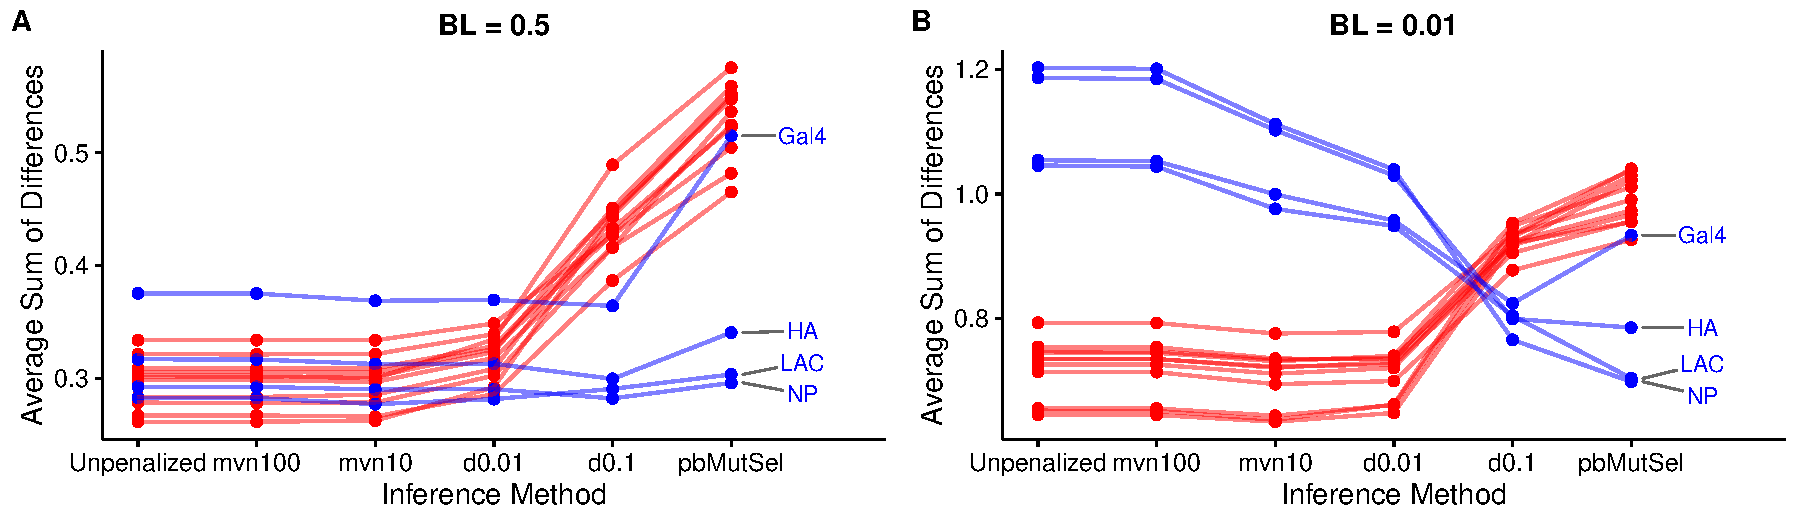
\includegraphics[width=7in]{SI_Figures/diffsum_lineplot.pdf}}
\noindent{\textbf{Figure S2} Sum of absolute differences between true and inferred stationary amino-acid frequencies.

\newpage
\vspace*{-0.75in}
\centerline{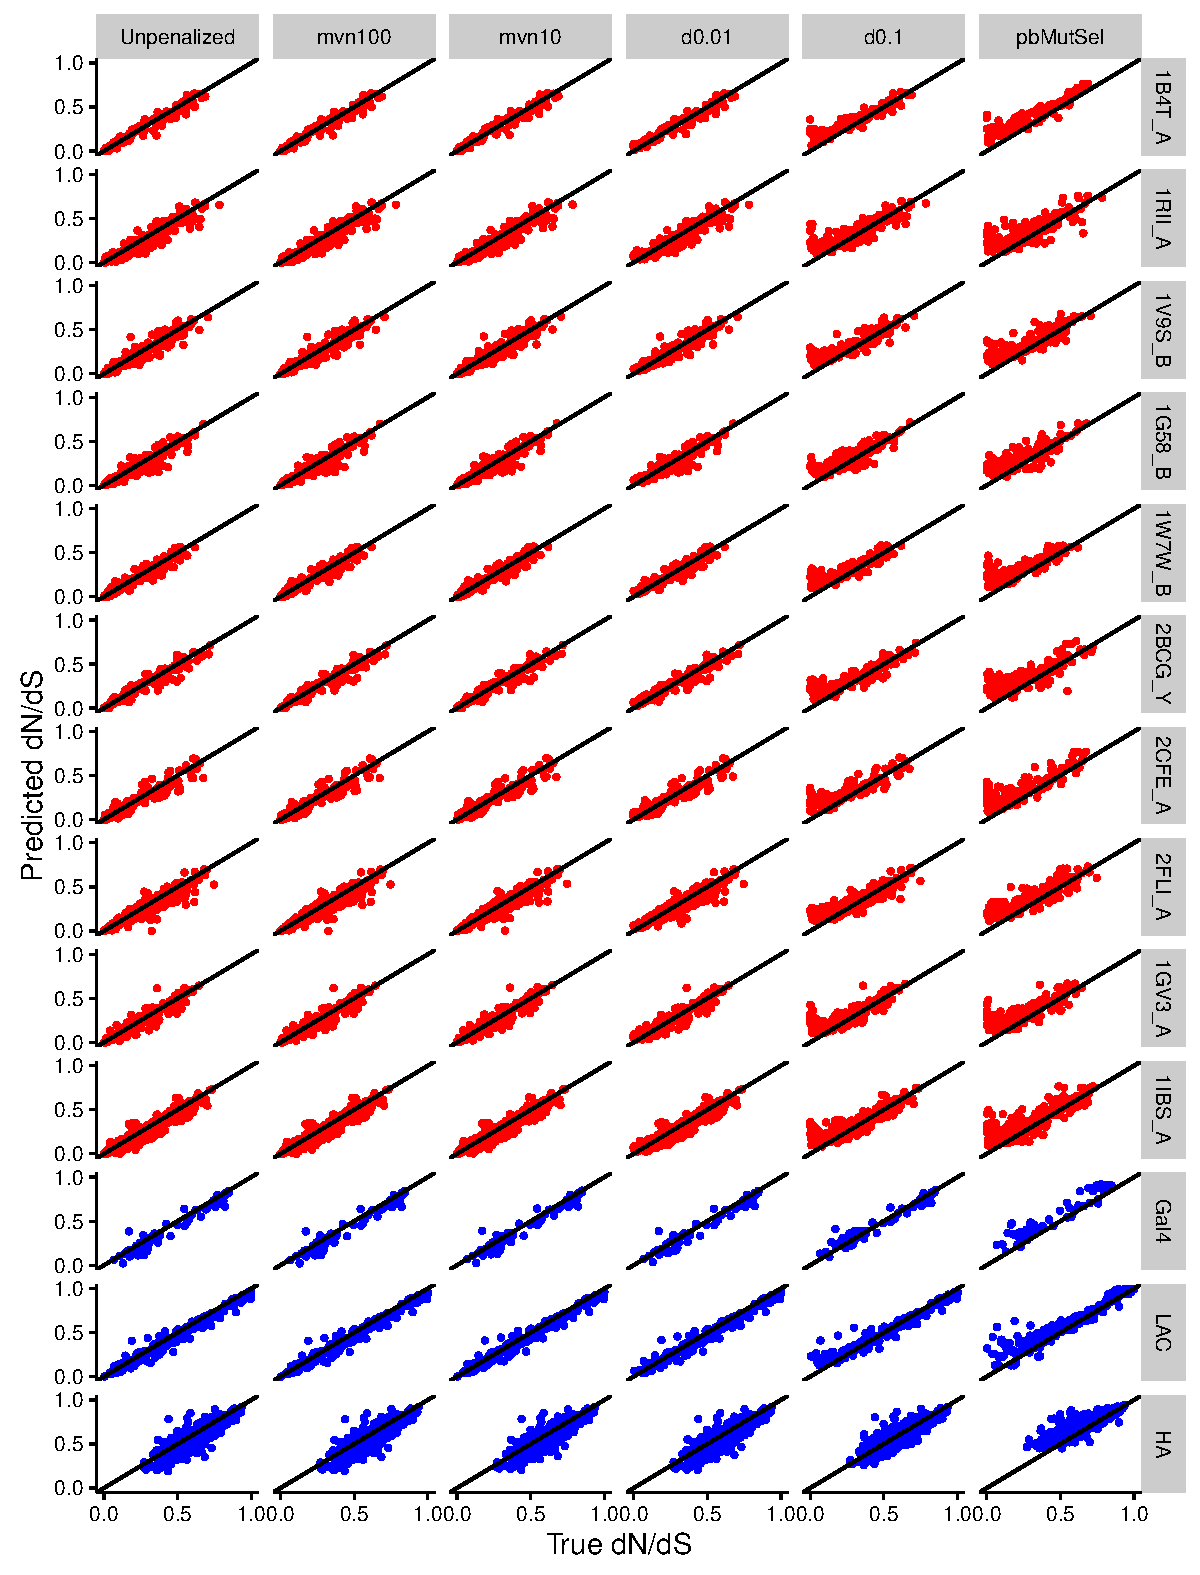
\includegraphics[width=7in]{SI_Figures/scatter_dnds_bl0_5_full.pdf}}
\noindent{\textbf{Figure S3} Scatterplots of predicted vs.\ true $dN/dS$ ratios, for all inference methods, across BL=0.5 simulations. Each line indicates the $y=x$ line.}

\newpage
\vspace*{-0.75in}
\centerline{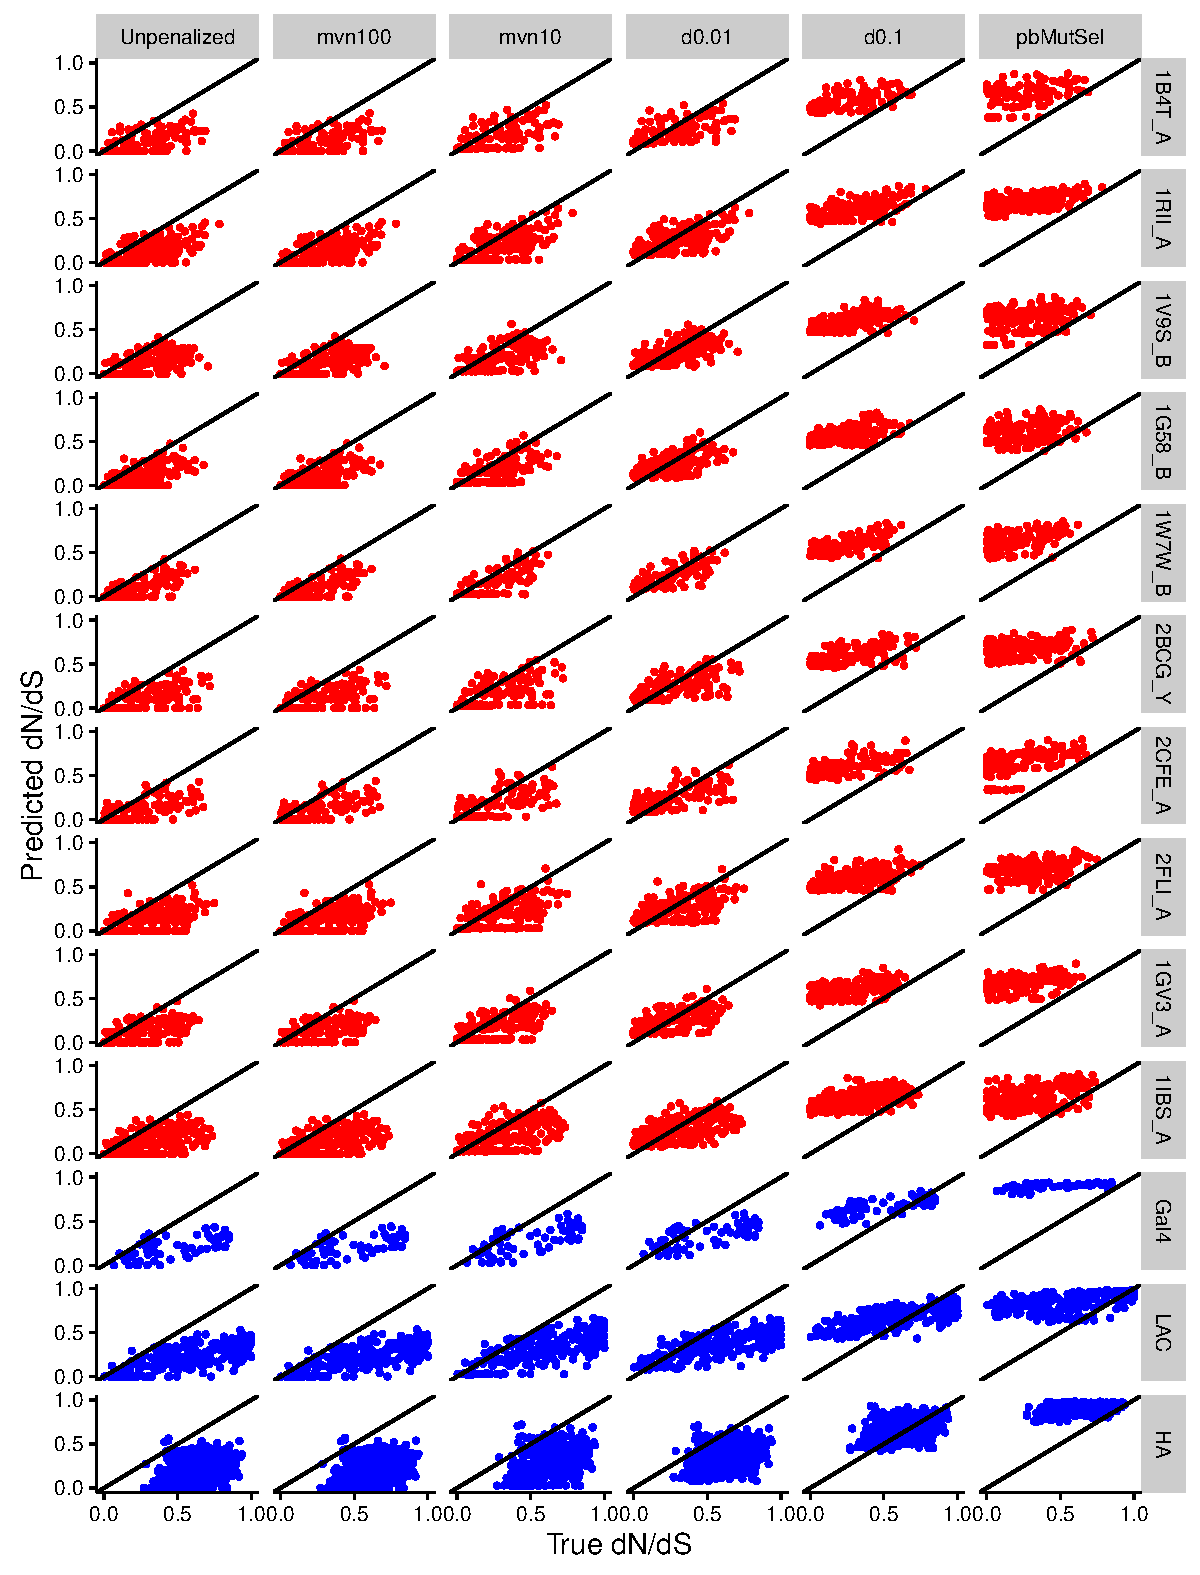
\includegraphics[width=7in]{SI_Figures/scatter_dnds_bl0_01_full.pdf}}
\noindent{\textbf{Figure S4} Scatterplots of predicted vs.\ true $dN/dS$ ratios, for all inference methods, across BL=0.01 simulations. Each line indicates the $y=x$ line.}

\newpage
\vspace*{-0.75in}
\centerline{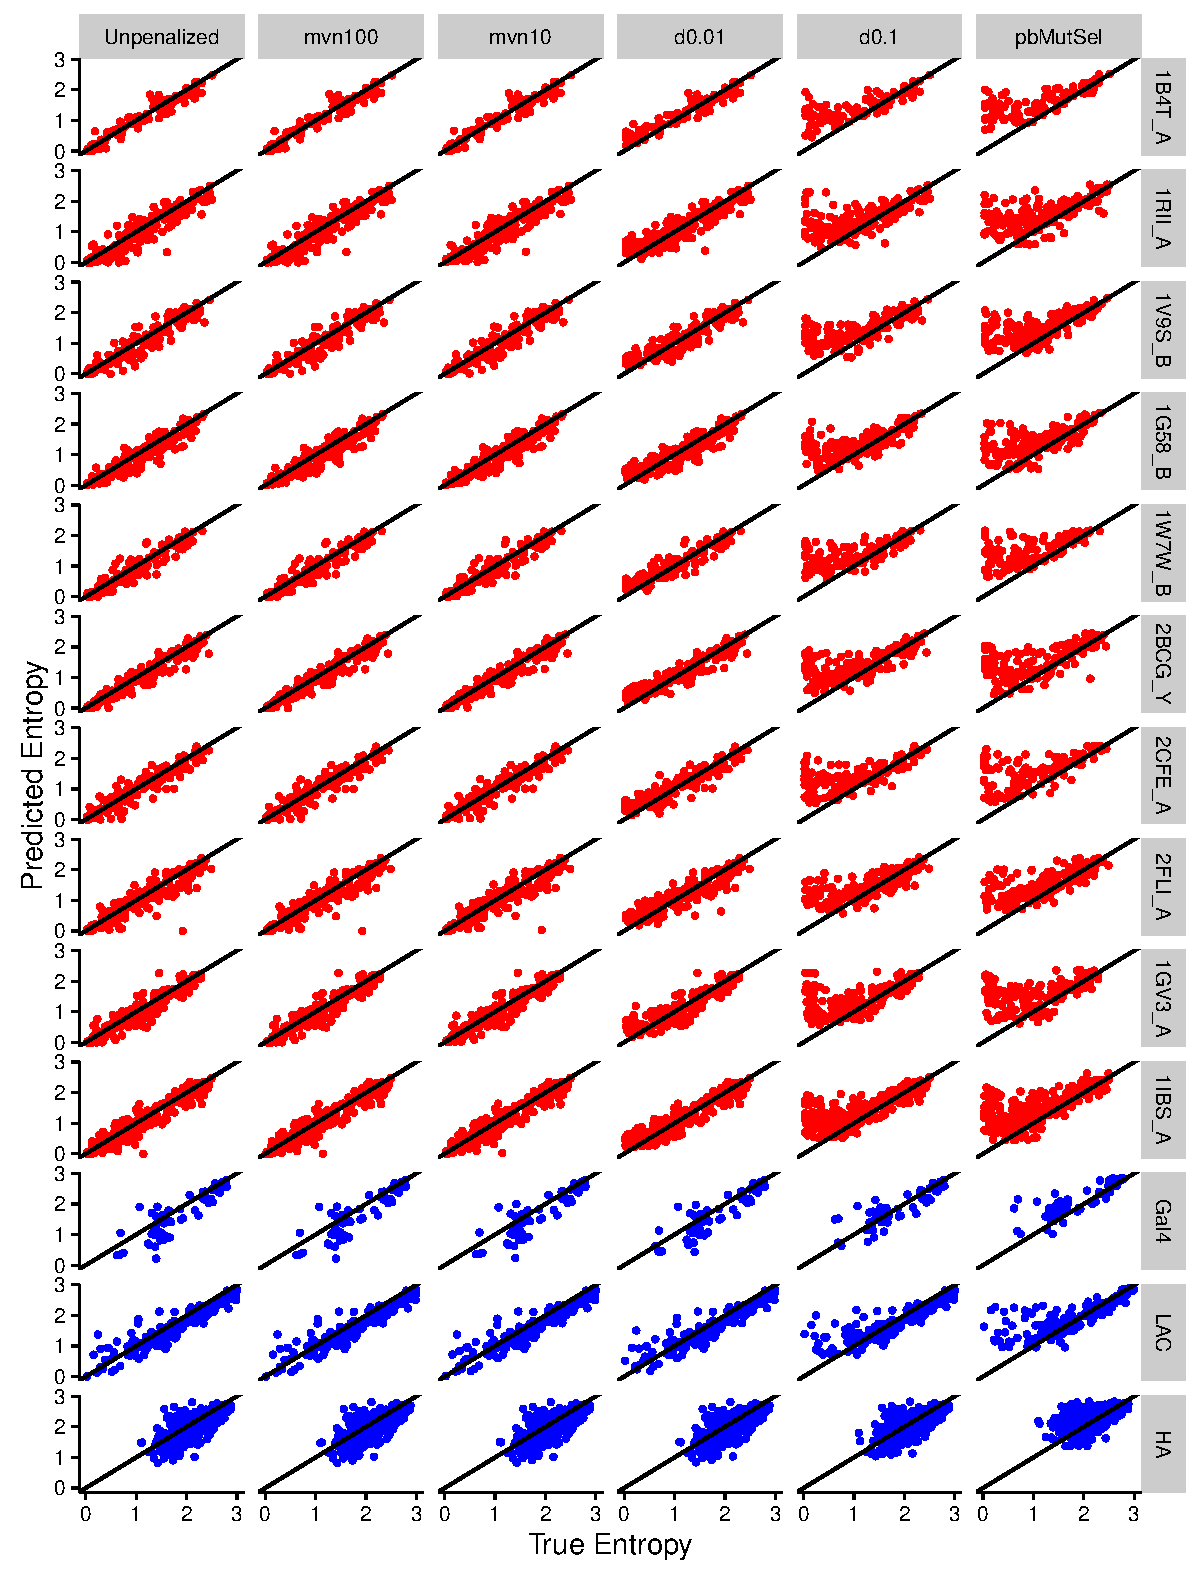
\includegraphics[width=7in]{SI_Figures/scatter_entropy_bl0_5_full.pdf}}
\noindent{\textbf{Figure S5} Scatterplots of predicted vs.\ true entropies, for all inference methods, across BL=0.5 simulations. Each line indicates the $y=x$ line.}

\newpage
\vspace*{-0.75in}
\centerline{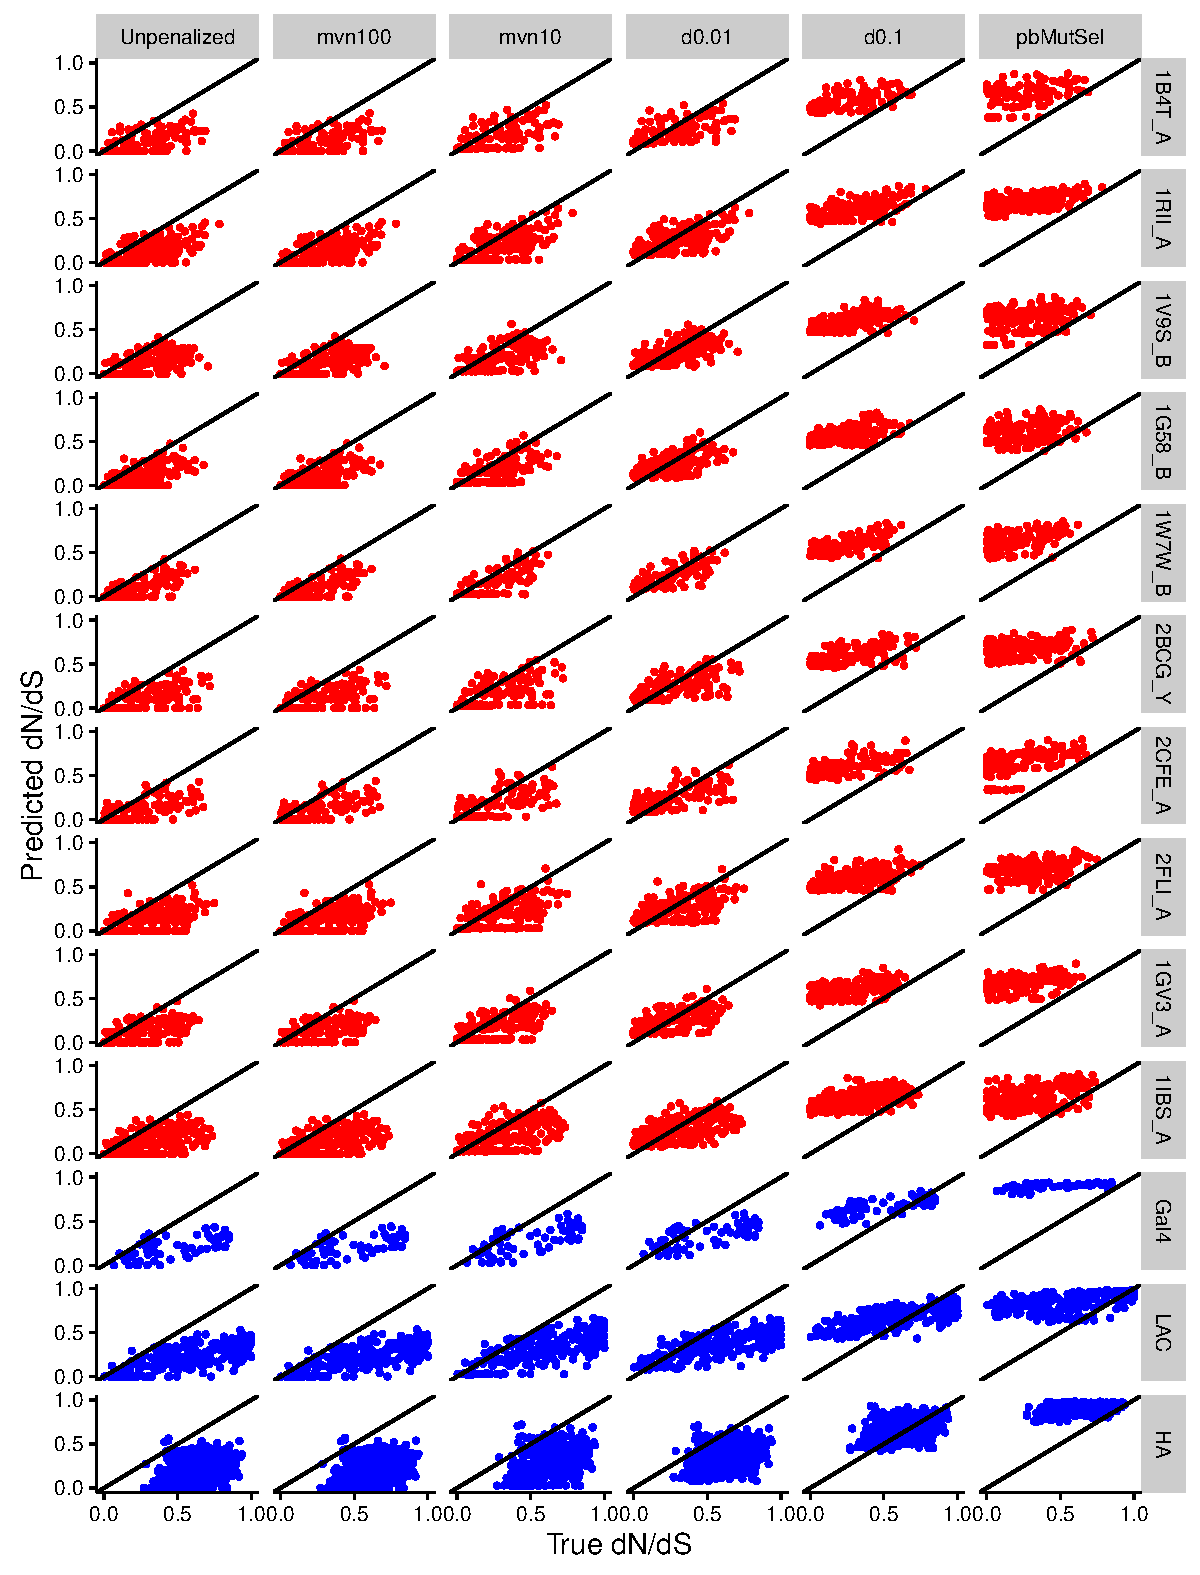
\includegraphics[width=7in]{SI_Figures/scatter_dnds_bl0_01_full.pdf}}
\noindent{\textbf{Figure S6} Scatterplots of predicted vs.\ true entropies, for all inference methods, across BL=0.01 simulations. Each line indicates the $y=x$ line.}

\newpage
\vspace*{-0.75in}
\centerline{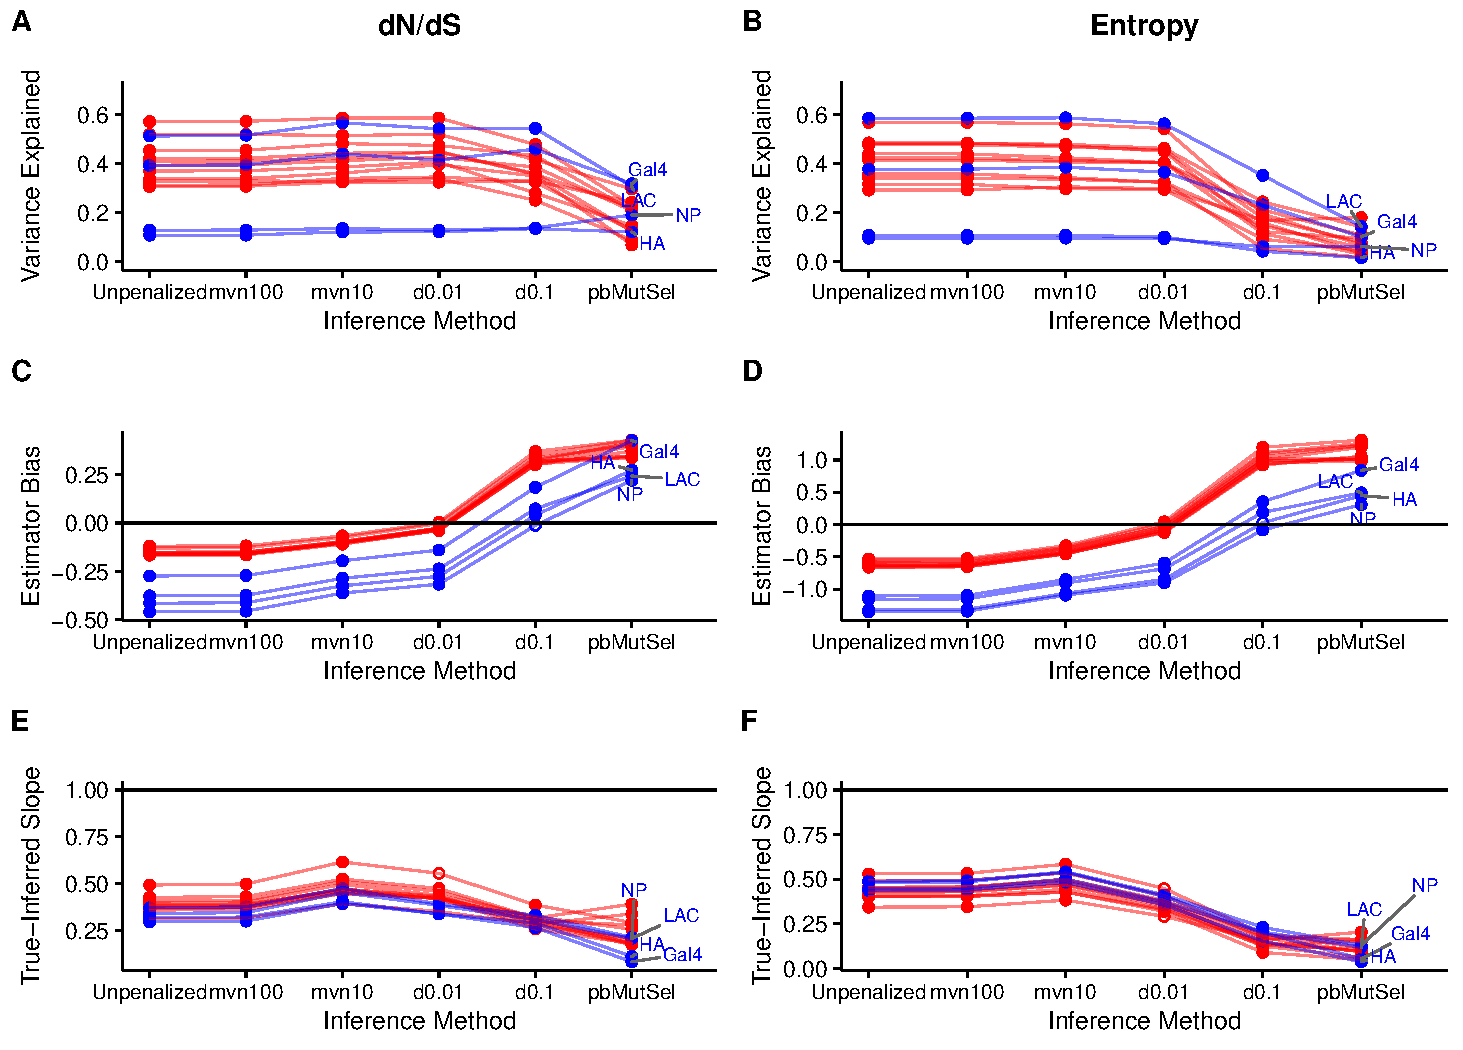
\includegraphics[width=7in]{SI_Figures/r2_bias_slope_bl0_01.pdf}}
\noindent{\textbf{Figure S7} Performance of mutation--selection model inference platforms for BL=0.01 simulations. (A-B) $r^2$ between true and inferred $dN/dS$ (A) and entropy (B) across inference methods, for all simulated datasets. (C-D) Estimator bias of inference methods relative to true $dN/dS$ (C) and entropy (D) values, for all simulated datasets. Open points indicate biases that were not significantly different from 0 (Bonferroni-corrected $P>0.05$, test for intercept in linear model), and solid points indicate biases that were significantly different from 0 (Bonferroni-corrected $P<0.05$). The straight line indicates an estimator bias of 0, meaning an unbiased predictor. Note that panels (C-D) use different y-axis ranges, due to the different scales between $dN/dS$ and entropy. (E-F) Slope for the linear relationship of inferred regressed on true $dN/dS$ (E) and entropy (F) values. Open points indicate slopes that were not significantly different from 1 (Bonferroni-corrected $P>0.05$, test for slope in linear model not equal to 1), and solid points indicate biases that were significantly different from 1 (Bonferroni-corrected $P<0.05$). The straight line indicates the null slope of 1.}

\newpage
\vspace*{-0.75in}
\centerline{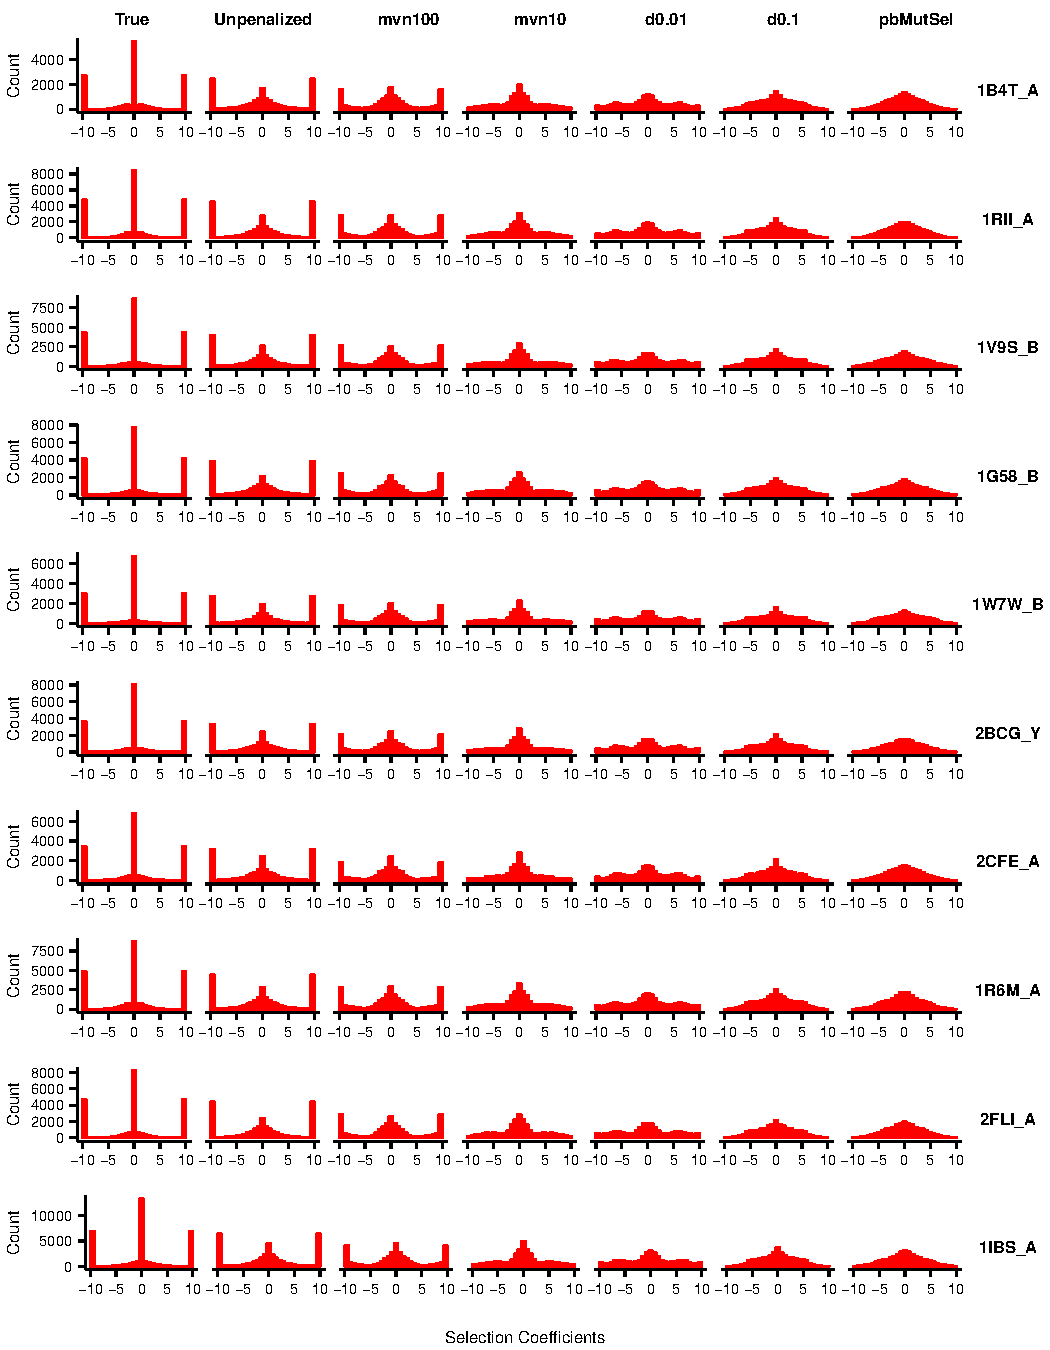
\includegraphics[width=7in]{SI_Figures/selcoeff_histograms_bl0_5.pdf}}
\noindent{\textbf{Figure S8} Distributions of scaled selection coefficients across all inference methods, for BL=0.5 simulations not shown in Figure 6. $S$ distributions shown represent the selection coefficients among all possible single-nucleotide changes, across all sites.}


\newpage
\vspace*{-0.75in}
\centerline{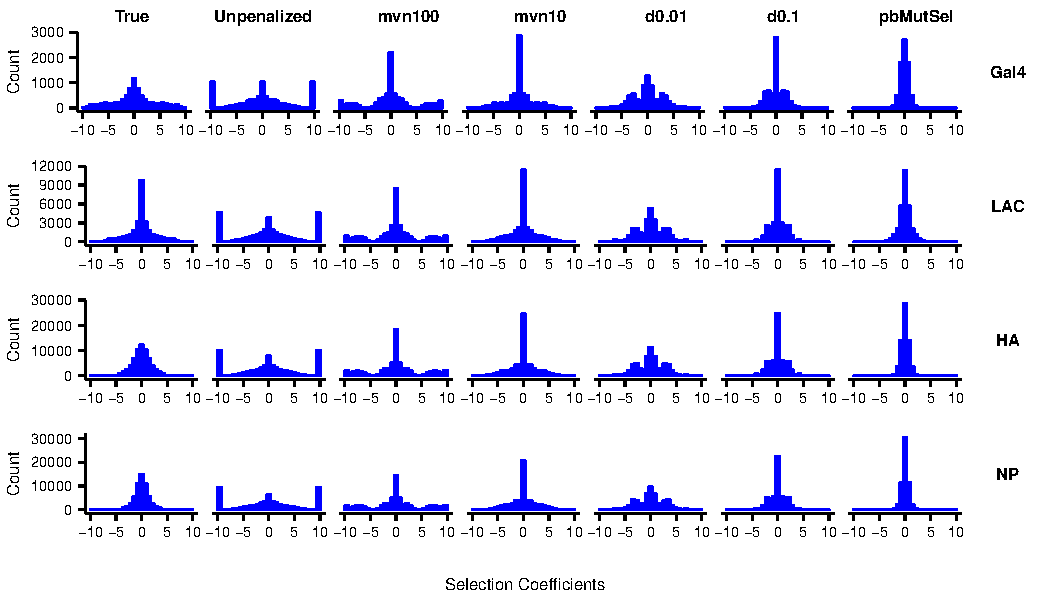
\includegraphics[width=7in]{SI_Figures/selcoeff_histograms_dms_bl0_01.pdf}}
\noindent{\textbf{Figure S9} Distributions of scaled selection coefficients across all inference methods, for BL=0.01 DMS simulations. $S$ distributions shown represent the selection coefficients among all possible single-nucleotide changes, across all sites.}

\newpage
\vspace*{-0.75in}
\centerline{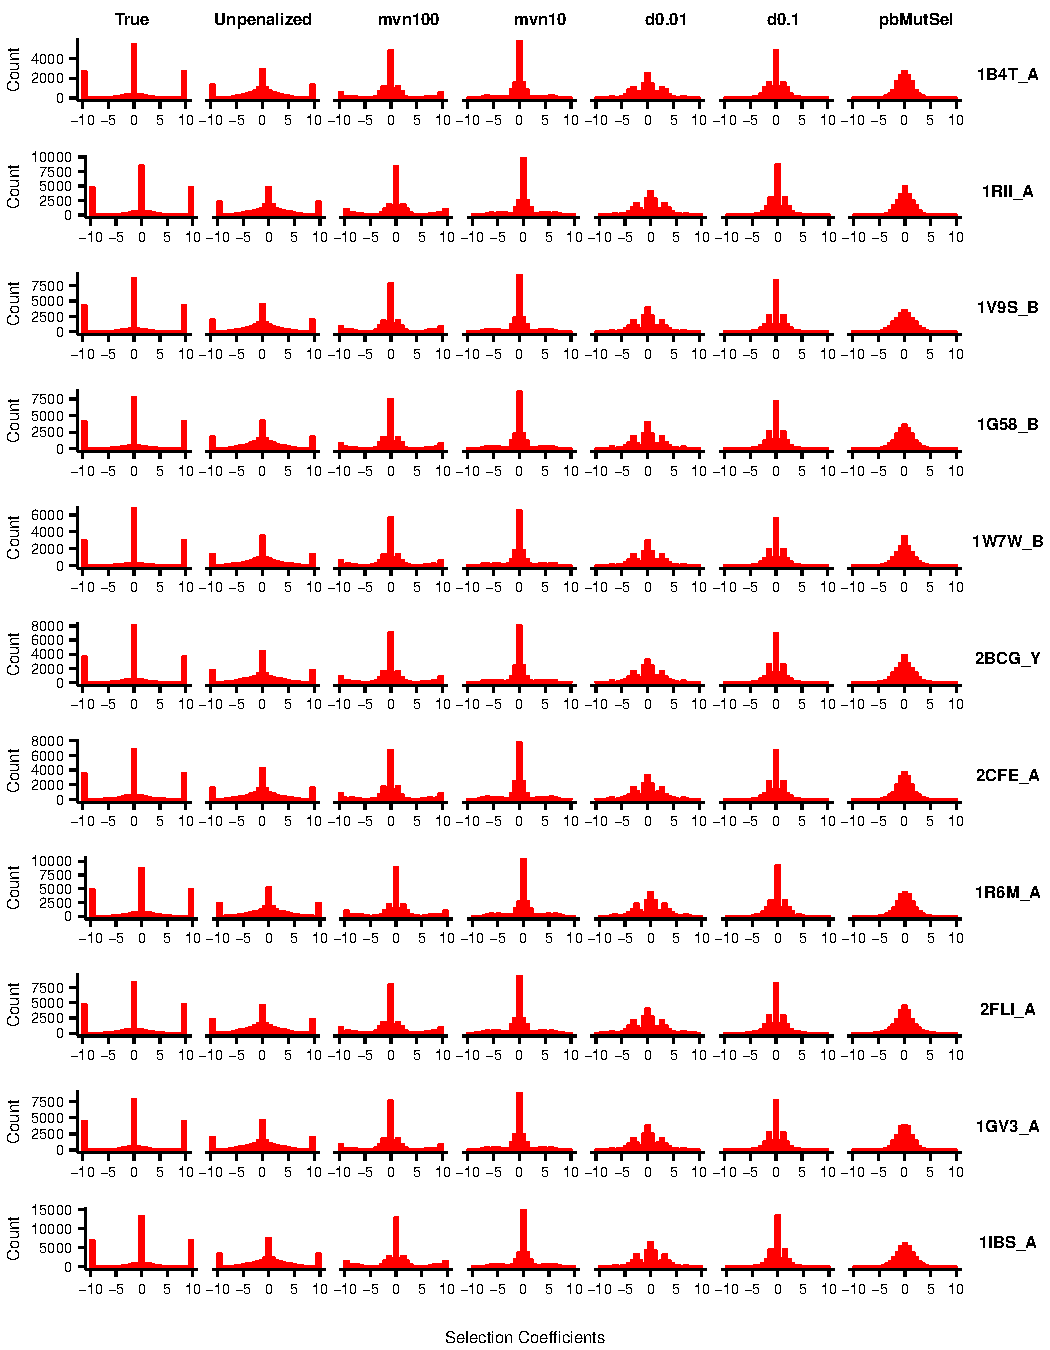
\includegraphics[width=7in]{SI_Figures/selcoeff_histograms_natural_bl0_01.pdf}}
\noindent{\textbf{Figure S10} Distributions of scaled selection coefficients across all inference methods, for BL=0.01 natural simulations. $S$ distributions shown represent the selection coefficients among all possible single-nucleotide changes, across all sites.}


\end{document}
